% Latex template: mahmoud.s.fahmy@students.kasralainy.edu.eg
% For more details: https://www.sharelatex.com/learn/Beamer

\documentclass[aspectratio=1610]{beamer}					% Document class

\setbeamertemplate{footline}[text line]{%
  \parbox{\linewidth}{\vspace*{-8pt}Establishing a quantitative framework for analyzing inducible gene expression in HeLa cells \hfill\insertshortauthor\hfill\insertpagenumber}}
\setbeamertemplate{navigation symbols}{}

\usepackage[english]{babel}				% Set language
\usepackage[utf8x]{inputenc}			% Set encoding

\mode<presentation>						% Set options
{
  \usetheme{default}					% Set theme
  \usecolortheme{default} 				% Set colors
  \usefonttheme{default}  				% Set font theme
  \setbeamertemplate{caption}[numbered]	% Set caption to be numbered
}

% Uncomment this to have the outline at the beginning of each section highlighted.
%\AtBeginSection[]
%{
%  \begin{frame}{Outline}
%    \tableofcontents[currentsection]
%  \end{frame}
\usepackage{graphicx}					% For including figures
\usepackage{booktabs}					% For table rules
\usepackage{hyperref}	
\usepackage{tikz-network}				% For cross-referencing
\usepackage[absolute,overlay]{textpos}
\usepackage{bm}
\usepackage[font=small,labelfont=bf]{caption}				% For cross-referencing

\title{Establishing a quantitative framework for analyzing inducible gene expression in HeLa cells}	% Presentation title
\author{Clayton W. Seitz}								% Presentation author
\date{\today}									% Today's date	

\begin{document}

% Title page
% This page includes the informations defined earlier including title, author/s, affiliation/s and the date
\begin{frame}
  \titlepage
\end{frame}


% The following is the most frequently used slide types in beamer
% The slide structure is as follows:
%
%\begin{frame}{<slide-title>}
%	<content>
%\end{frame}


\begin{frame}{Interferon-$\gamma$ induces differential expression of many genes}

\vspace{0.1in}
Single cell transcriptome measurements of polyA mRNA for naïve HeLa cells (N=90), induced with interferon gamma (50ng/mL) for 24h

\begin{figure}
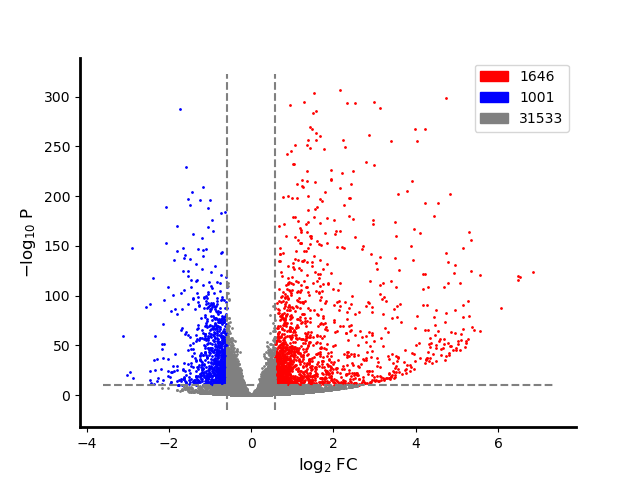
\includegraphics[width=7cm]{volcano.png}
\end{figure}

{\tiny Siwek et al. 
\it{Activation of Clustered IFN$\gamma$ Target Genes Drives Cohesin-Controlled Transcriptional Memory} Cell 2020}

This is just a birds eye view of whats really going on...

\end{frame}

\begin{frame}

\end{frame}

\begin{frame}{Promoter models are necessary for non-constitutive gene expression}


\begin{textblock*}{7cm}(1cm,1cm)
\begin{figure}
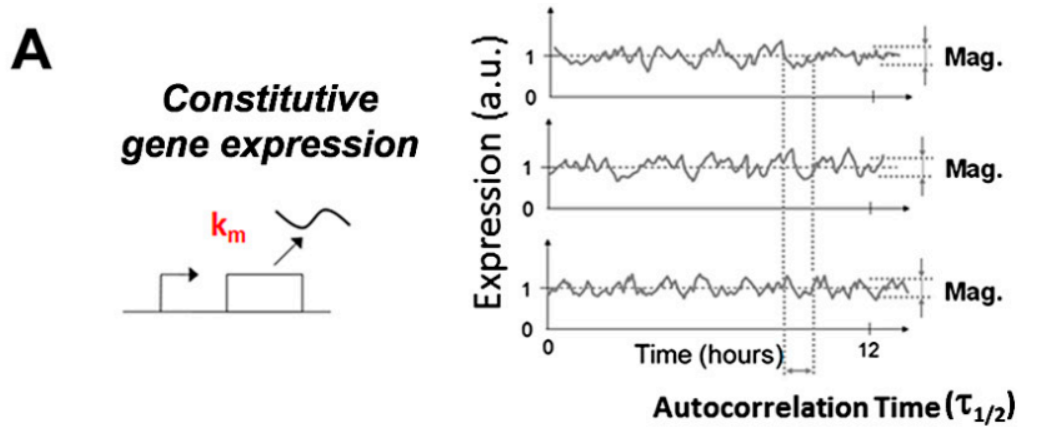
\includegraphics[width=7cm]{burst-1.png}
\end{figure}
\end{textblock*}

\begin{textblock*}{7cm}(8cm,1cm)
\begin{figure}
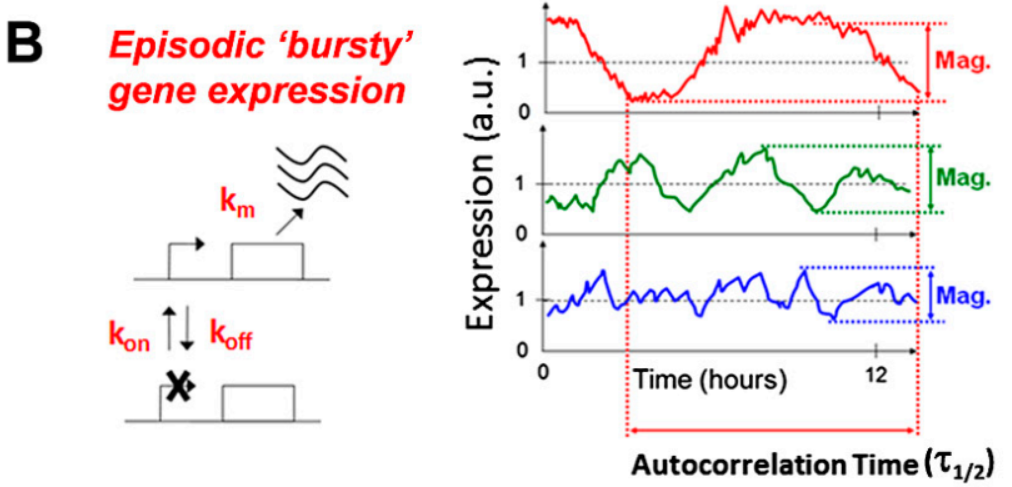
\includegraphics[width=6cm]{burst-2.png}
\end{figure}
\end{textblock*}


\begin{textblock*}{6cm}(1cm,5cm)
\hspace{0.5in}\textbf{Single-state models}
\begin{itemize}
\item RNAs are 'born' at a fixed rate
\item RNA counts are Poisson
\end{itemize}
\end{textblock*}

\begin{textblock*}{6cm}(8cm,5cm)
\hspace{0.5in}\textbf{Multi-state models}
\begin{itemize}
\item Promoter can be in multiple states (switching behavior)
\item RNA counts are not Poissonian
\end{itemize}

\end{textblock*}

\begin{textblock*}{15cm}(0.5cm,8cm)
Single-state models tend to \textcolor{red}{underestimate variance in RNA counts}
\end{textblock*}


\end{frame}



\begin{frame}{Gene expression is stochastic (live-cell MS2-MCP)}
\begin{figure}
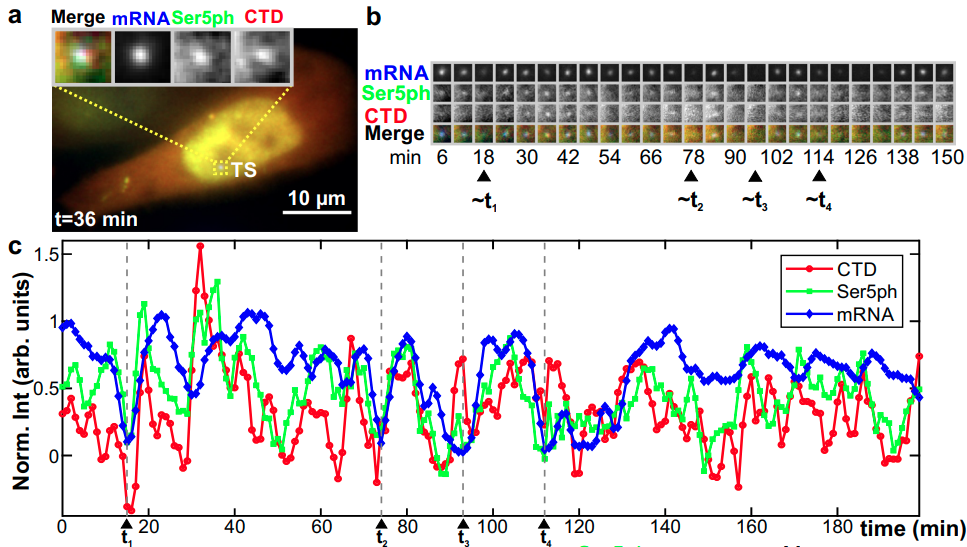
\includegraphics[width=12cm]{live-cell.png}
\end{figure}
{\tiny Forero-Quintero, et al. \textit{Live-cell imaging reveals the spatiotemporal organization of endogenous RNAPII phosphorylation at a single gene}. Nat Commun 2021}\\
\end{frame}



\begin{frame}{Example: variability in STL1 mRNA counts per cell at 0.4M NaCl}

\begin{textblock*}{5cm}(3.25cm,0.5cm)
\begin{figure}
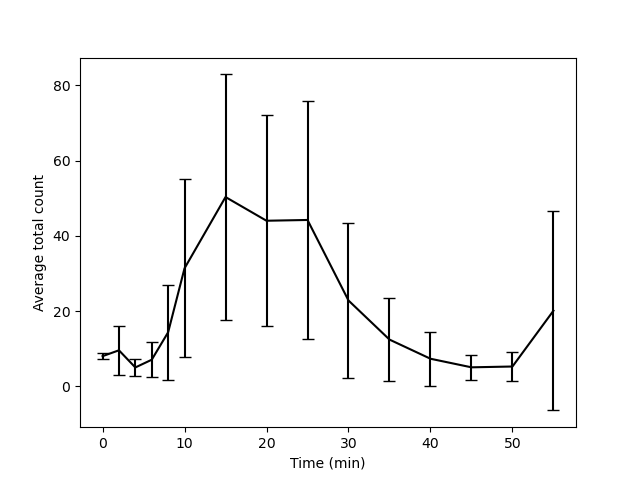
\includegraphics[width=10cm]{avg-count.png}
\end{figure}
\end{textblock*}

\vspace{7.25cm}
Error bars represent standard deviations from the mean\\
Cells marked ON for $>$ 3 STL1 mRNA in yeast

\end{frame}


\begin{frame}{Assessing STL1 mRNA count variability at the transcription site}

\begin{textblock*}{5cm}(0.75cm,1.5cm)
\begin{itemize}
\item Brightest spot in the nucleus defined as putative TS
\item TS marked ACTIVE if $I>2*\mathrm{med}$
\item Nascent mRNA count is $\mathrm{round}(I/\mathrm{med})$
\item Count variability suggests asynchrony
\end{itemize}

\end{textblock*}

\begin{textblock*}{5cm}(7cm,0.75cm)
\begin{figure}
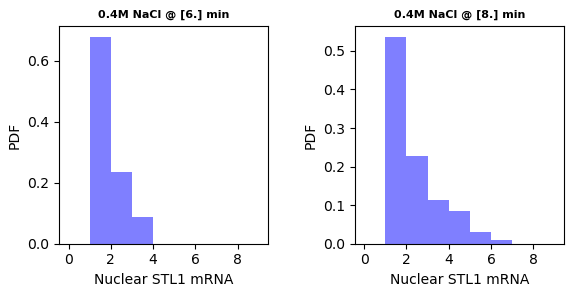
\includegraphics[width=8cm]{active-ts-dist-2.png}
\end{figure}
\end{textblock*}

\begin{textblock*}{5cm}(7cm,4.5cm)
\begin{figure}
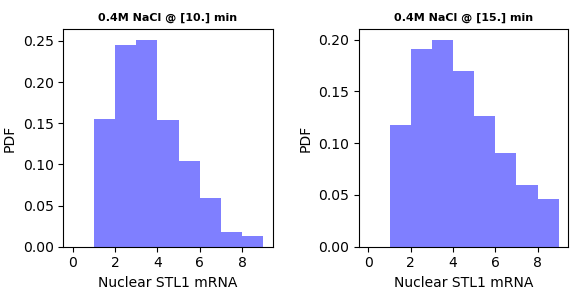
\includegraphics[width=8cm]{active-ts-dist-1.png}
\end{figure}
\end{textblock*}

\end{frame}


\begin{frame}{A spatial model for induced gene expression}

Let $X$ represent an arbitrary RNA transcript of an induced gene $G$. Assume two promoter states (on and off)

\begin{align*}
\mathrm{Gene\;activation}: G_{off} &\overset{k_{on}}{\rightarrow} G_{on}\\
\mathrm{Gene\;inactivation}: G_{on} &\overset{k_{off}}{\rightarrow} G_{off}\\
\mathrm{Transcription}: G_{on} &\overset{k_{t}}{\rightarrow} G_{on} + X_{\mathrm{nuc}}\\
\mathrm{RNA \;Export}: X_{\mathrm{nuc}} &\overset{k_{exp}}{\rightarrow} X_{\mathrm{cyt}}\\
\mathrm{RNA\; degradation}: X_{\mathrm{cyt}} &\overset{\gamma}{\rightarrow} \emptyset\\
\end{align*}

Raw data collected post induction can be used to infer parameters

\begin{equation*}
\theta = \left( k_{on},k_{off},k_{t},k_{exp},\gamma\right)
\end{equation*}

\end{frame}

\begin{frame}{Bayesian inference of model parameters}

It is well-known that using just means and variances gives poor estimates of the model parameters (Munsky et al. PNAS 2018)\\
\vspace{0.2in}
Let $\theta = \left( k_{on},k_{off},k_{t},k_{exp},\gamma\right)$. Using Bayes Rule: 

\begin{align*}
P(\theta|X) = \frac{P(X|\theta)P(\theta)}{\int P(X|\theta)P(\theta)} \propto P(X|\theta)P(\theta)
\end{align*}

Can infer $\theta$ if we know the likelihood $P(X|\theta)$ (the hard part) and specify a prior $P(\theta)$\\
\vspace{0.2in}
Generally we have to resort to Monte Carlo methods to find $P(X|\theta)$

\end{frame}

\begin{frame}{Kolmogorov's forward equation (chemical master equation)}

Dynamics on biochemical reaction networks are inherently stochastic and the state space is discrete. We can only write probabilities over the state space

\vspace{0.1in}

\begin{align*}
P(\mathbf{x}_{i},t) &= \sum_{j} T_{ji}(\mathbf{x}_{i},t|\mathbf{x}_{j},t-\Delta t)P(\mathbf{x}_{j},t-\Delta t)\\ 
&= \sum_{k} T_{k}(\mathbf{x}_{i},t|\mathbf{x}_{i}-\nu_{k},t-\Delta t)P(\mathbf{x}_{i}-\nu_{k},t-\Delta t)
\end{align*}

where $T_{k}$ is the probability of a reaction channel $k$ firing in the interval $(t,t+\Delta t)$.\\
\vspace{0.1in}
Taking the limit $\Delta t \rightarrow 0$ one can derive the forward Kolmogorov equation or chemical master equation (CME)

\begin{align*}
\frac{dP(\mathbf{x},t|\mathbf{x}_{0})}{dt} = \sum_{k} T_{k}(\mathbf{x}-\nu_{k})P(\mathbf{x}-\nu_{k},t) - T_{k}(\mathbf{x})P(\mathbf{x},t)
\end{align*}

\end{frame}




\end{document}